%% Version 4.3.2, 25 August 2014
%
%%%%%%%%%%%%%%%%%%%%%%%%%%%%%%%%%%%%%%%%%%%%%%%%%%%%%%%%%%%%%%%%%%%%%%
% Template.tex --  LaTeX-based template for submissions to the 
% American Meteorological Society
%
% Template developed by Amy Hendrickson, 2013, TeXnology Inc., 
% amyh@texnology.com, http://www.texnology.com
% following earlier work by Brian Papa, American Meteorological Society
%
% Email questions to latex@ametsoc.org.
%
%%%%%%%%%%%%%%%%%%%%%%%%%%%%%%%%%%%%%%%%%%%%%%%%%%%%%%%%%%%%%%%%%%%%%
% PREAMBLE
%%%%%%%%%%%%%%%%%%%%%%%%%%%%%%%%%%%%%%%%%%%%%%%%%%%%%%%%%%%%%%%%%%%%%

%% Start with one of the following:
% DOUBLE-SPACED VERSION FOR SUBMISSION TO THE AMS
%\documentclass{ametsoc}

% TWO-COLUMN JOURNAL PAGE LAYOUT---FOR AUTHOR USE ONLY
 \documentclass[twocol]{ametsoc}

%%%%%%%%%%%%%%%%%%%%%%%%%%%%%%%%
%%% To be entered only if twocol option is used

\journal{mwr}

%  Please choose a journal abbreviation to use above from the following list:
% 
%   jamc     (Journal of Applied Meteorology and Climatology)
%   jtech     (Journal of Atmospheric and Oceanic Technology)
%   jhm      (Journal of Hydrometeorology)
%   jpo     (Journal of Physical Oceanography)
%   jas      (Journal of Atmospheric Sciences)	
%   jcli      (Journal of Climate)
%   mwr      (Monthly Weather Review)
%   wcas      (Weather, Climate, and Society)
%   waf       (Weather and Forecasting)
%   bams (Bulletin of the American Meteorological Society)
%   ei    (Earth Interactions)

%%%%%%%%%%%%%%%%%%%%%%%%%%%%%%%%
%Citations should be of the form ``author year''  not ``author, year''
\bibpunct{(}{)}{;}{a}{}{,}

%%%%%%%%%%%%%%%%%%%%%%%%%%%%%%%%

%%% To be entered by author:

%% May use \\ to break lines in title:

\title{Physics-dynamics coupling with element-based high-order Galerkin methods: quasi equal-area physics grid}

%%% Enter authors' names, as you see in this example:
%%% Use \correspondingauthor{} and \thanks{Current Affiliation:...}
%%% immediately following the appropriate author.
%%%
%%% Note that the \correspondingauthor{} command is NECESSARY.
%%% The \thanks{} commands are OPTIONAL.

    %\authors{Author One\correspondingauthor{Author One, 
    % American Meteorological Society, 
    % 45 Beacon St., Boston, MA 02108.}
% and Author Two\thanks{Current affiliation: American Meteorological Society, 
    % 45 Beacon St., Boston, MA 02108.}}

\authors{Peter H. Lauritzen\correspondingauthor{Climate and Global Dynamics, National Center for Atmospheric Research, 1850 Table Mesa Drive, Boulder, Colorado, USA.}}

%% Follow this form:
    % \affiliation{American Meteorological Society, 
    % Boston, Massachusetts.}

\affiliation{Climate and Global Dynamics, National Center for Atmospheric Research, 1850 Table Mesa Drive, Boulder, Colorado, USA.}

%% Follow this form:
    %\email{latex@ametsoc.org}

\email{pel@ucar.edu}

%% If appropriate, add additional authors, different affiliations:
\extraauthor{Mark A. Taylor}
\extraaffil{Sandia National Laboratories, Albuquerque, New Mexico, USA.}
\extraauthor{Paul A. Ullrich}
\extraaffil{Department of Land, Air and Water Resources, University of California, Davis, California, USA}
\extraauthor{Julio T. Bacmeister}
\extraaffil{Climate and Global Dynamics, National Center for Atmospheric Research, 1850 Table Mesa Drive, Boulder, Colorado, USA.}
\extraauthor{Steve Goldhaber}
\extraaffil{Climate and Global Dynamics, National Center for Atmospheric Research, 1850 Table Mesa Drive, Boulder, Colorado, USA.}

%% May repeat for a additional authors/affiliations:

%\extraauthor{}
%\extraaffil{}

%%%%%%%%%%%%%%%%%%%%%%%%%%%%%%%%%%%%%%%%%%%%%%%%%%%%%%%%%%%%%%%%%%%%%
% ABSTRACT
%
% Enter your abstract here
% Abstracts should not exceed 250 words in length!
%
% For BAMS authors only: If your article requires a Capsule Summary, please place the capsule text at the end of your abstract
% and identify it as the capsule. Example: This is the end of the abstract. (Capsule Summary) This is the capsule summary. 

\abstract{Enter the text of your abstract here.}

\begin{document}

%% Necessary!
\maketitle


%%%%%%%%%%%%%%%%%%%%%%%%%%%%%%%%%%%%%%%%%%%%%%%%%%%%%%%%%%%%%%%%%%%%%
% MAIN BODY OF PAPER
%%%%%%%%%%%%%%%%%%%%%%%%%%%%%%%%%%%%%%%%%%%%%%%%%%%%%%%%%%%%%%%%%%%%%
%

%% In all cases, if there is only one entry of this type within
%% the higher level heading, use the star form: 
%%
\begin{itemize}
\item We should compute TKE of tendencies and show that we ar removing scales with nc<2
\end{itemize}
\section{Introduction}
An increasing number of numerical methods publications in the atmospheric science literature concern transport, shallow-water, and three-dimensional models employing element-based high-order Galerkin discretizations such as finite-element and discontinuous Galerkin methods \citep[for an introduction to these methods see, e.g., ][]{Durran,NLL2011LNCSE}. Some global models based on Galerkin methods have reached a level of maturity for which they are being considered for next generation climate and weather models due to their inherent conservation properties, high-order accuracy (for smooth problems), high parallel efficiency, high processor efficiency, and geometric flexibility facilitating mesh-refinement applications. NCAR's Community Atmosphere Model \citep[CAM; ][]{CAM5} offers a dynamical core based on continuous Galerkin finite elements \citep{TF2010JCP}, referred to as CAM-SE \citep[CAM Spectral Elements; ][]{DetAl2012IJHPCA,TES2008JPCS}. CAM-SE is, in particular, being used for high resolution climate modeling \citep[e.g., ][]{JAME:JAME20125} and static mesh-refinement applications \citep{FT2004MWR,ZJT2013,ZetAl2014JC,GetAl2014GMD}. Other examples of models based on high-order Galerkin methods that are being considered for `operational' weather-climate applications are \citet{Giraldo20083849}, \citet{NCT2009CF} and \citet{BSBDK2013TCFD}.


\begin{figure}[t]
\noindent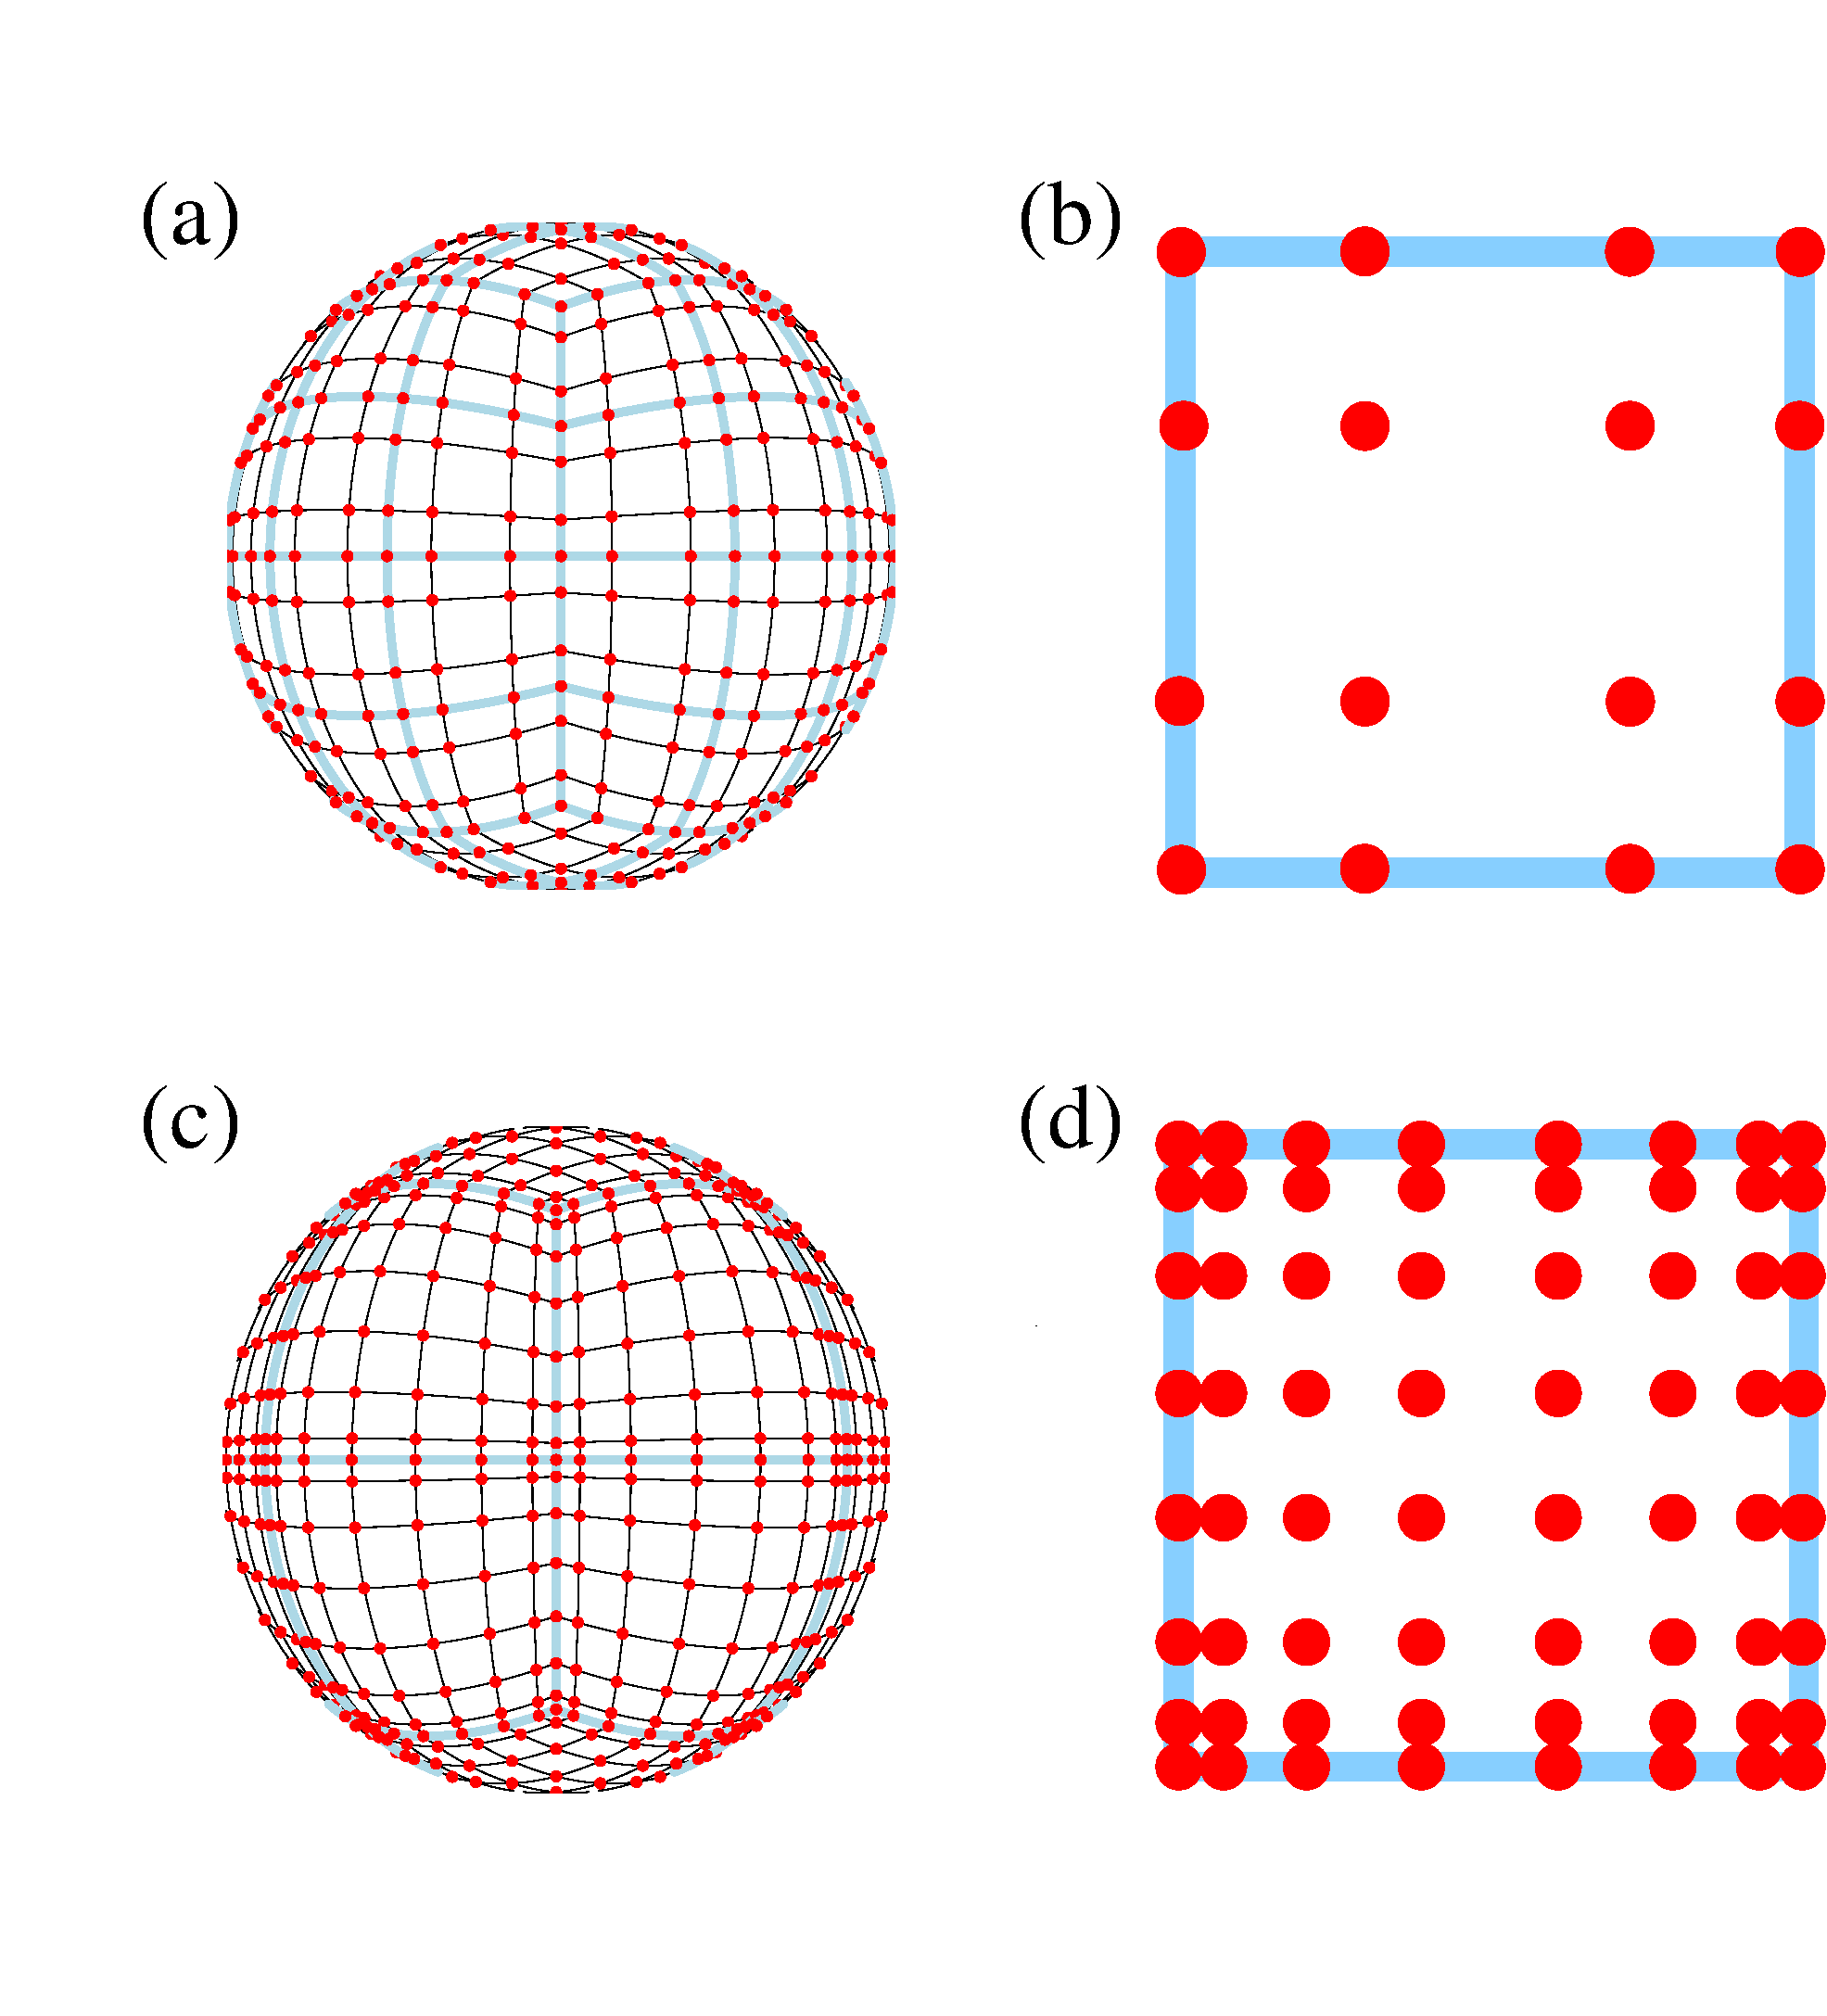
\includegraphics[width=19pc,angle=0]{figs/quadrature-fig/gll.pdf}\\
\caption{Example of CAM-SE GLL quadrature grids, marked with red filled circles, (a \& c) on the cubed-sphere and (b \& d) in an element. (a)-(b) and (c)-(d) use $4\times 4$ ($np=4$) and $8\times 8$ ($np=8$) GLL quadrature points in each element, respectively. (a) and (c) have the same average grid-spacing at the Equator (7.5$^\circ$) which is obtained by using (a) $4\times 4$ ($ne=4$) and (b) $2\times 2$ ($ne=2$) elements on each cubed-sphere face/panel, respectively. The element boundaries are marked with thick light blue lines. The grid configurations shown on (a) and (c) are referred to as $ne4np4$ and $ne2np8$, respectively.}
\label{fig:gll-grids}
\end{figure}

Traditionally the state of the atmosphere passed to the sub-grid-scale parameterizations (also referred to as {\em{physics}}) for models based on finite-volume and finite-difference methods has been the cell-averaged state in each control volume and the grid-point value, respectively. For the regular latitude-longitude, cubed-sphere and icosahedral grids the distance between the grid-points is gradually varying for finite-volume/finite-difference discretizations. If the same physics-dynamics coupling paradigm is applied to high-order element-based Galerkin methods, the state of the atmosphere passed to physics would be evaluated at the quadrature points. In the case of CAM-SE that would be the Gauss-Lobatto-Legendre (GLL) quadrature points. Having the physics and dynamics grids coincide is obviously convenient since no interpolation is needed (which could disrupt conservation properties) and the number of degrees of freedom on both grids is exactly the same. However, for high-order quadrature rules the quadrature points are not globally or locally equi-spaced. For example, Figure \ref{fig:gll-grids} shows GLL points on the cubed-sphere and in an element for degree 3 ($np=4$ quadrature points) and degree 7 ($np=8$ quadrature points) Lagrange polynomial basis in CAM-SE. Both grids have the same average resolution on the sphere (due to different number of elements), however, the higher the order of the quadrature rule the less equi-distant are the quadrature points. GLL quadrature points cluster near the edges and, in particular, the corners of the elements.

\begin{figure}[t]
\noindent\includegraphics[width=19pc,angle=0]{figs/se_gll_cv_grid.eps}\\
\caption{An example of control volumes constructed around GLL quadrature points (NE4NP4) so that the spherical area of the control volumes exactly match the quadrature weight multiplied by the metric factor.}
\label{fig:cv-grids}
\end{figure}

\begin{figure}[t]
\noindent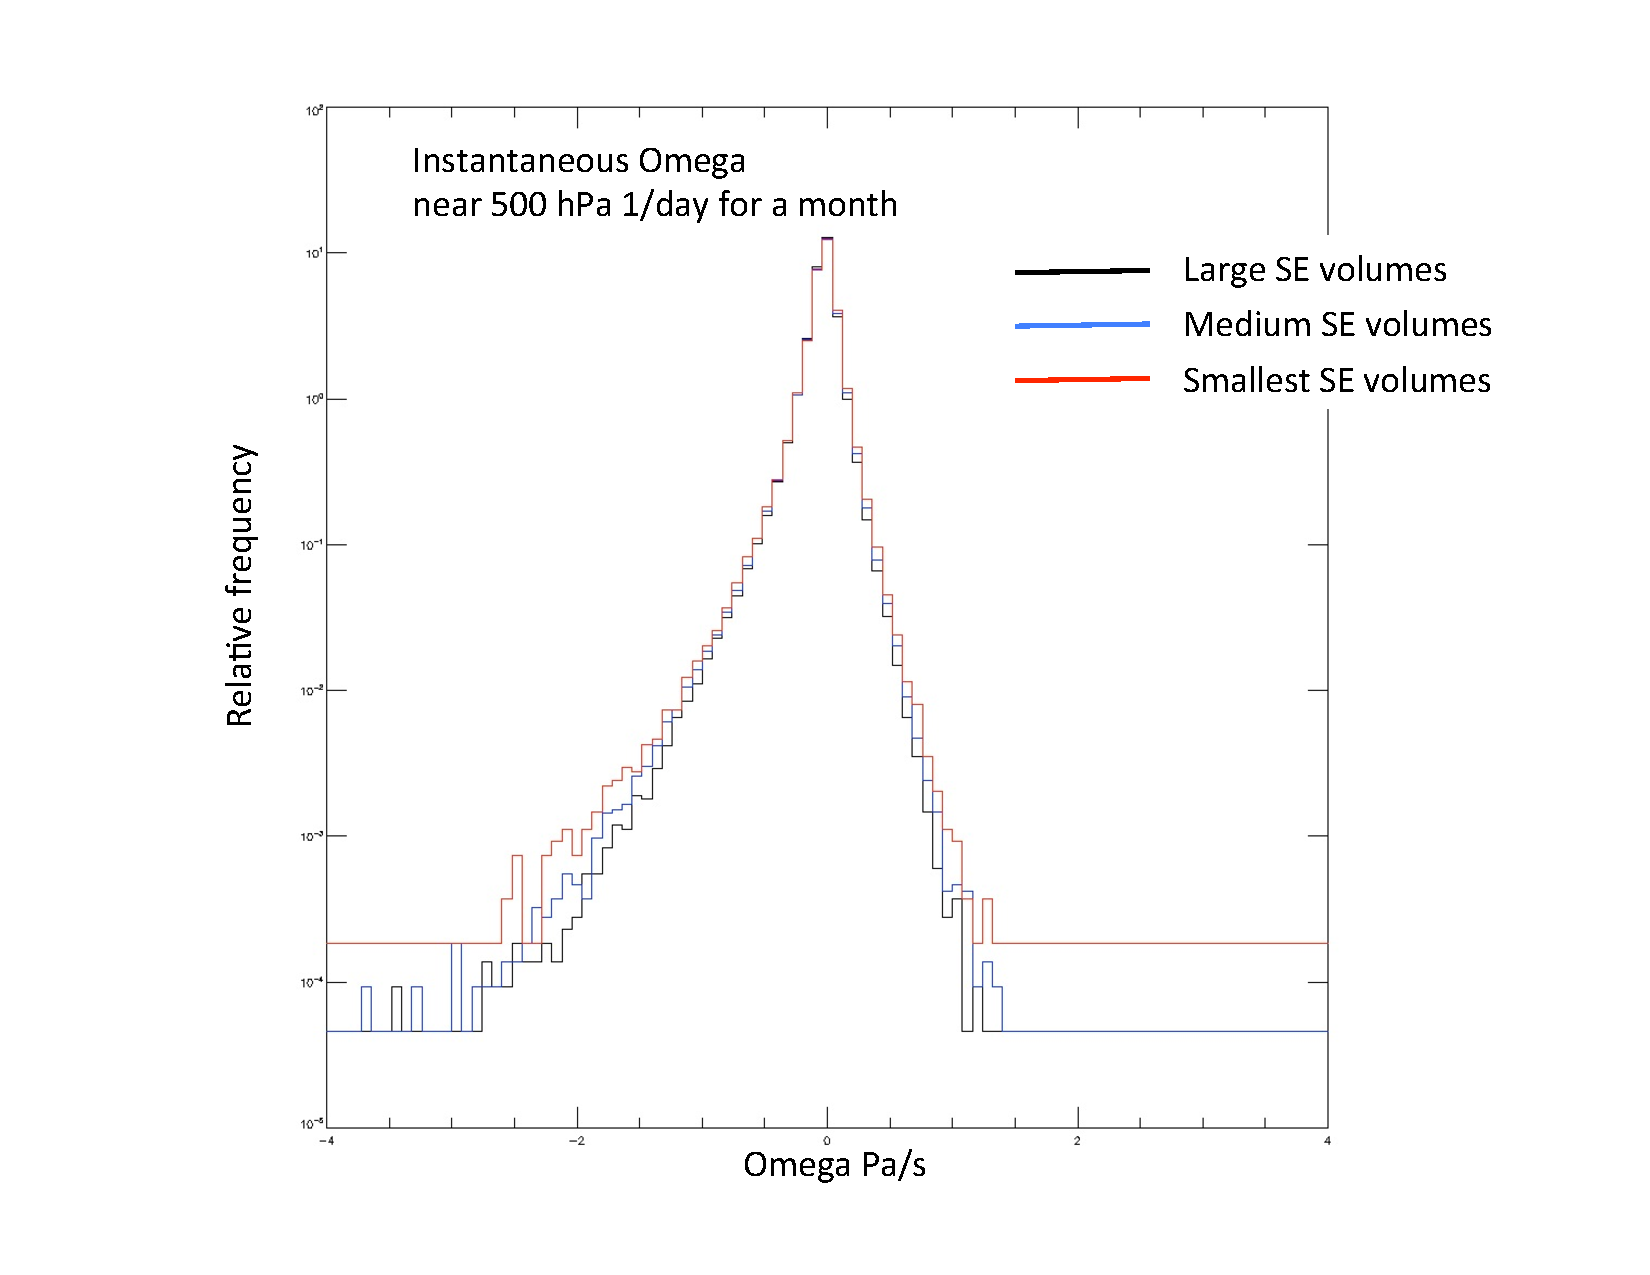
\includegraphics[width=19pc,angle=0]{figs/omega-se-volumes.pdf}\\
\caption{PDF of instantaneous $\omega$ (1 month) classifying the points into small, medium, and large volumes/GLL 
weights. Note the consistent higher $omega$ values for smaller areas compared to $\omega$ associated with larger volumes (which makes sense). The question is how parameterizations respond to that.}\label{fig:omega-se-volumes}
\end{figure}

Parameterizations use the state of the atmosphere from the dynamical core as the large-scale state for computing sub-grid-scale processes. For example, the dynamical core state defines the large-scale environment in a mass-flux based convection scheme. One may think of the dynamical core state as the average state of the atmosphere over a control volume as is inherent in finite-volume methods. For finite-difference methods the point value is thought of as representative for the atmospheric state in the vicinity of the point value and one can usually associate a volume with the grid-point. Hence the physics grid (the grid on which the state of the atmosphere is evaluated and passed to physics) and the dynamics grid (the grid the dynamical core uses) coincide. If we apply this concept to GLL quadrature values then a volume associated with the quadrature point should be defined. An example of that is shown on Figure \ref{fig:cv-grids} where control volumes have been defined around the quadrature points so that the spherical area of the control volumes exactly match the Gaussian weight multiplied by the metric term (these weights are used for integrating the basis functions over the elements and can therefore, in this context, be interpreted as areas). [{\color{red}{Mark: could we be mathematically more rigorous? perhaps an appendix describing the iterative algorithm?}}] This grid is used in the NCAR CESM (Community Earth System Model) coupler for passing states between ocean, atmosphere and land-ice components since the current remapping method is finite-volume based and therefore requires control volumes {\footnote{it is noted that methods exist that do not require control volumes for conservative interpolation \citep{UT2015MWR}}}. Hence the components `see' an irregular atmospheric grid. Similarly, the parameterizations in the atmosphere `see' a state that is anisotropically sampled in space \citep[see Figure 1 and 5 in ][]{KetAl2008JGR}. Figure \ref{fig:omega-se-volumes} show a PDF of instantaneous vertical velocity $\omega$ for a one month `AMIP'-like simulation with CAM-SE. The vertical velocity has been classified into small, medium and large areas/GLL weights. Consistently $\omega$ is higher for smaller areas, which makes sense, however, the question is how physics responds to that.


\begin{figure*}[t]
\noindent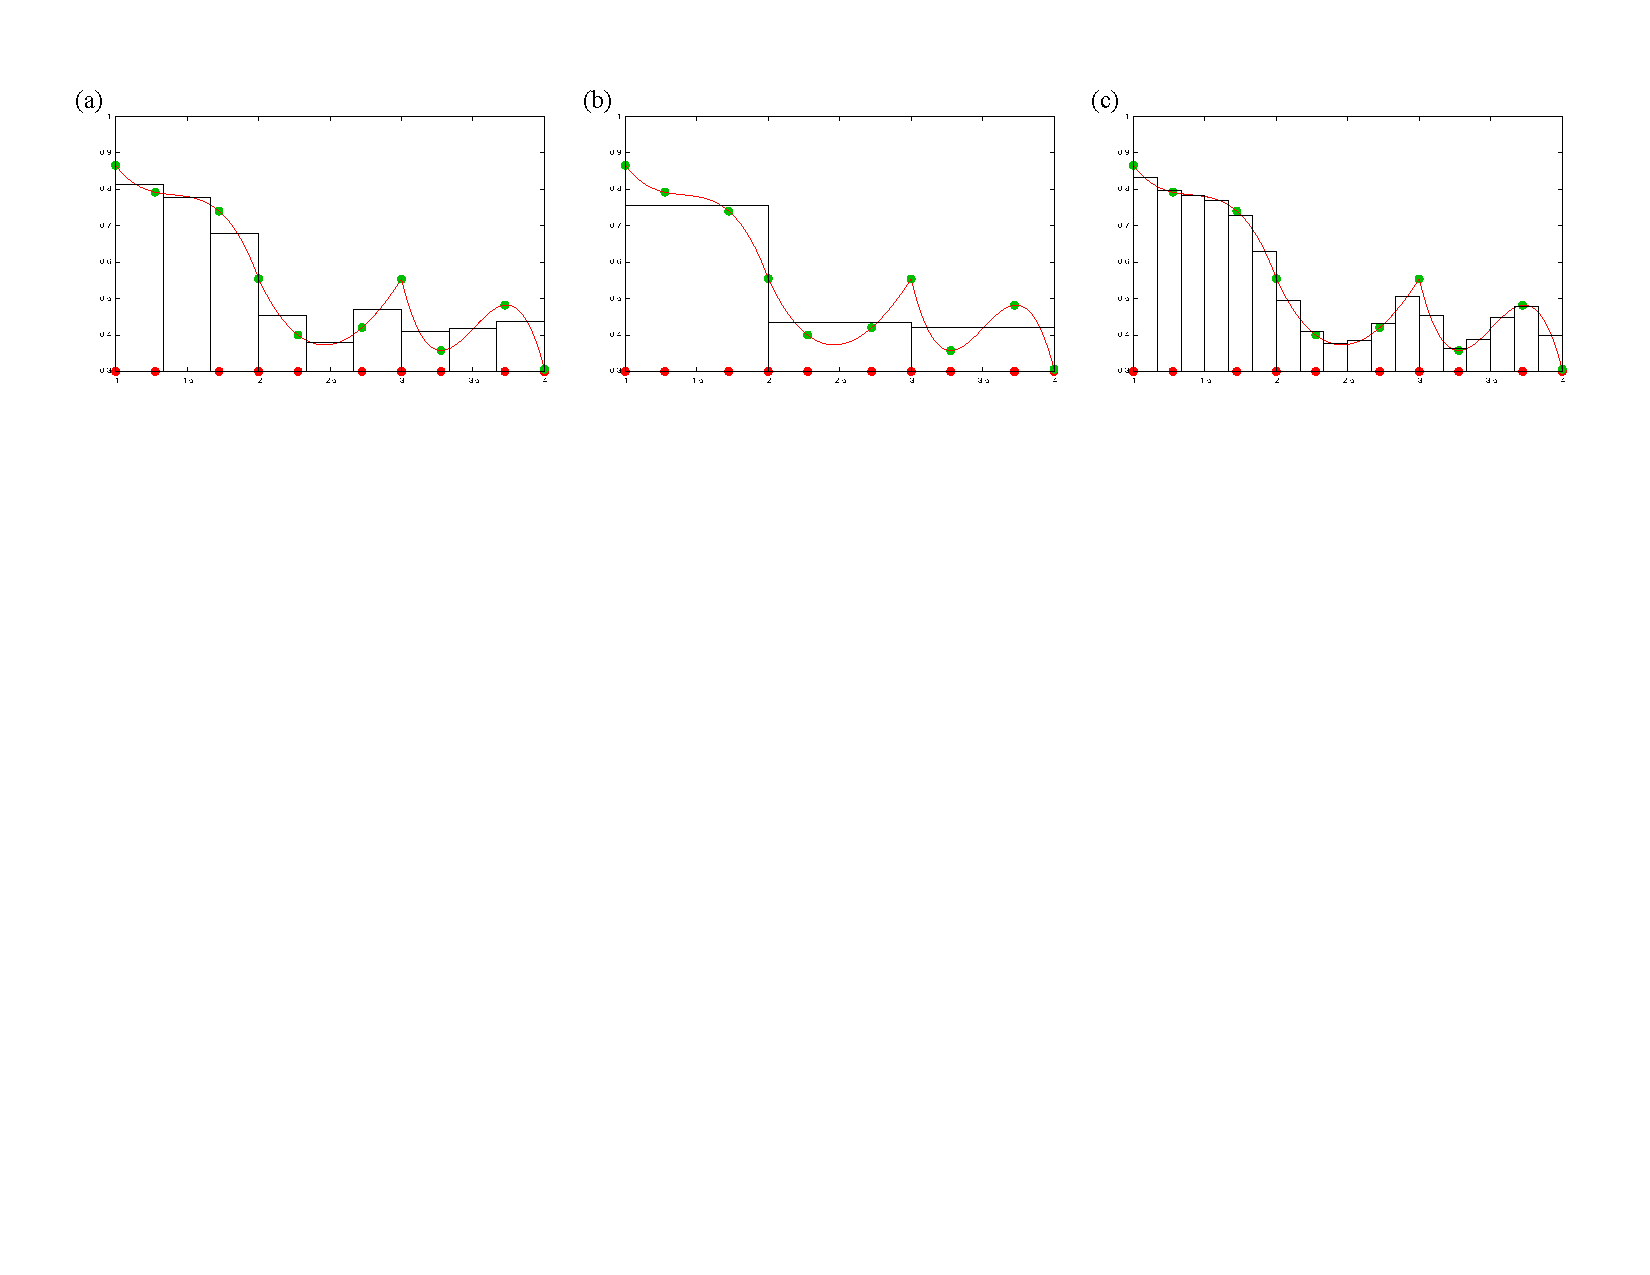
\includegraphics[width=38pc,angle=0]{figs/physgrid-1d.pdf}\\
\caption{A graphical illustration of the physics grid in one dimension. Three elements are shown and the filled red circles are the GLL quadrature points in each element. The red curve is the basis function representation of the field and the green filled circles are the quadrature point values. The physics grid divides each element into equal-area control volumes. On the Figure each element is divided into (a) 3, (b) 1 and (c) 6 control volumes, respectively. The histogram shows the average values over the physics grid control volumes resulting from integrating the basis functions over the respective control volumes.}
\label{fig:physgrid-1d}
\end{figure*}

The quadrature grid in high-order element-based Galerkin methods is defined to perform mathematical operations on the basis functions, e.g., computing gradients and integrals, rather than evaluating the state variables for physics-dynamics coupling. Within each element there is a high-order $C^{\infty}$ representation of state variables. One may argue that it would be more consistent to integrate the basis functions over quasi-equal area control volumes within each element and pass those control volume average values to physics rather than irregularly spaced quadrature point values (see Figure \ref{fig:physgrid-1d}).  

\begin{figure*}[t]
\noindent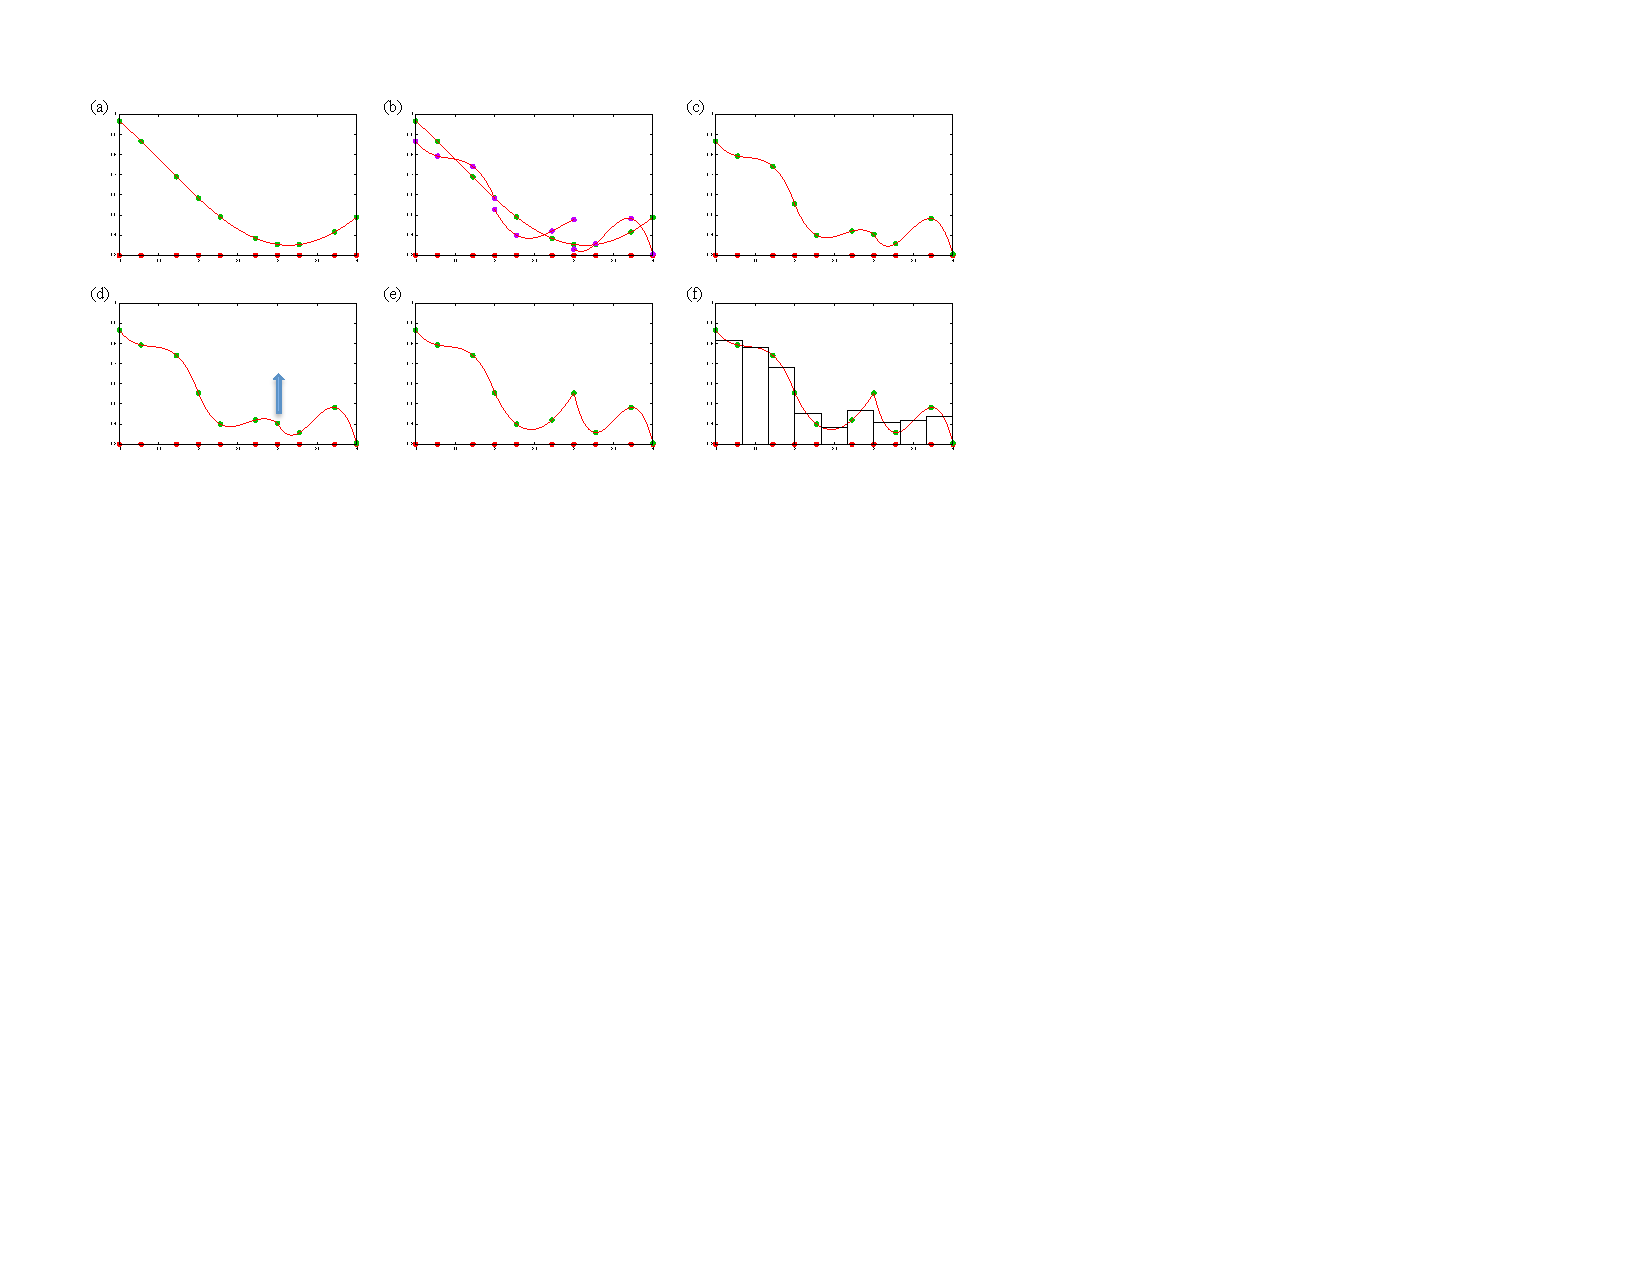
\includegraphics[width=38pc,angle=0]{figs/se-schematic.pdf}\\
\caption{A 1D schematic illustration on how CAM-SE advances the solution to the equations of motion in time. Consider 3 elements. The red filled circles are the GLL quadrature points in each element ($np=4$). Note that the quadrature points on the boundary are shared between elements. (a) Assume a degree 3 global Lagrange polynomial initial condition (red curve) which can be represented exactly by the degree 3 Lagrange basis in each element. (b) The solution to the equations of motion are advanced in time (one Runga-Kutta step) independently in each element leading to the quadrature values marked with filled purple circles. The Lagrange basis is shown with red curves connecting the purple circles. There are now two solutions, one from left and one from right, for the quadrature points at the element end points. In CAM-SE the values are averaged so that the solution is $C^0$. Note that the averaging changes the Lagrange polynomials throughout except at the internal quadrature points. (c) shows the solution after averaging. (d) Assume there is a grid-scale forcing that increases the quadrature value located at $x=3$. (e) The solution is now clearly $C^0$ at the element boundary at $x=3$. (f) Histogram shows the average values resulting in integrating the basis functions over the control volumes.}
\label{fig:se-schematic}
\end{figure*}

Integrating basis functions over control volumes may be beneficial in reducing the intrinsic oscillatory behavior of high-order basis functions within each element. Moreover, if there is a strong grid-scale forcing or oscillatory behavior near an element boundary, the solution will be least smooth near that element boundary. This is illustrated in the context of CAM-SE on Figure \ref{fig:se-schematic}. In this case when integrating basis functions over control volumes a grid-cell average value is more representative of the values near the extrema at the element boundary than the quadrature point value.

When introducing a physics grid separate from the dynamics grid the question arises of what the resolution of the physics grid should be compared to the dynamics grid. For example, Figure \ref{fig:physgrid-1d} shows physics grids with the same, coarser and finer resolution than the GLL dynamics grid. From linear stability and accuracy analysis of numerical methods, it is a common result that the shortest resolvable wavelengths are not accurately represented. Similar arguments can be made from analyzing total kinetic energy spectra \citep{S2011LNCSE}. One may therefore argue that only believable scales should be passed to the physical parameterizations \citep{LH1997MWR}, i.e. a coarser resolution physics grid. This concept was investigated in a spectral transform model by \cite{W1999T}. On the other hand, computing physics tendencies on a higher-resolution grid compared to the dynamical core may provide a better sampling of the atmospheric state, somewhat similar to the super-parameterization \citep{G2001JAS,GRL:GRL14999,SA2007ASL} and sub-columns{\footnote{\citet{gmdd-8-5041-2015} in the context of CAM}} \citep{subcolumn,JGRD:JGRD10481} concepts. This approach was taken by \cite{M2009T} in the context of vertical refinement. \cite{W2014PTRSL} found improved forecast scores by increasing the grid-point space resolution compared to the resolution in wave-number space for the spectral transform model at ECMWF. 

%Alternatively, one could combine the two ideas and compute the state of the atmosphere on a coarser resolution grid and then use sub-columns or super-parameterization. One thereby passes believable scales to the sub-grid scale model and thereby assumes that a statistical sampling, in the case of sub-columns, or a simplified cloud-resolving model, in the case of super-parameterization, provides a more accurate sub-grid-scale tendency than sampling the Galerkin basis functions over the sub-grid-scale. [Discuss \cite{W2014PTRSL}: spectral truncation and physics (physical) grid (see page 10; conclusions)]




%Separating physics and dynamics grids has been investigated in the context of spectral transform models by \citet{TELA:TELA0009}, in which the separation was performed by truncation in wavenumber space. Parts of the physical parameterizations (microphysics) were separated in \citet{JGRD:JGRD50711} and vertical grid separation was investigated in \citet{TELA:TELA394}. In this study we run all of the parameterization on the physgrid.


%In the context of spectral transform model \citet{TELA:TELA0009} held the physics forcing scale fixed while refining the horizontal resolution of the dynamical core. In the context of microphysics \citet{JGRD:JGRD50711} did a scale separation and \citet{TELA:TELA394} separated the vertical grids. While \citet{LH1997MWR} and \citet{TELA:TELA0009} separated scales truncation of the the wave transform, we here separate scales through integrating basis functions over control volumes and , contrary to \citet{JGRD:JGRD50711}, all of the physical parameterization computations are performed on the physgrid. We focus on horizontal separation of scales here.

{\color{red}{It is the purpose of this paper to formulate the CAM-SE-physgrid version in which we separate physics and dynamics grids as illustrated in one dimension above. We show simulations from Held-Suarez .... CAM5 aquaplanet. ...}}



% \subsection*{subsection}
% text...
\section{Methods}
Here we focus on CAM-SE, however, in principle the methods apply to any element-based high-order Galerkin model. The physics grid in CAM-SE is defined by sub-dividing each element using equi-angular gnomonic coordinate lines to define the sides of the physics grid control volumes. Note that the element boundaries are defined by equi-angular gnomonic grid lines.  The notation $nc=3$ refers to the configuration where the elements are divided into $nc\times nc=3\times 3$ quasi equal-area physics grid cells (see Figure \ref{fig:grids}). Defining the physics grid by sub-diving elements makes it possible to use the same infrastructure as used for the quadrature point values thereby facilitating its implementation in CAM-SE. Here we make use of the $NE30NP4$, $NE30NP4NC2$, $NE30NP4NC3$, and $NE30NP4NC4$ grids that use GLL quadrature point physics grid (physics and dynamics grid coincide), coarser ($nc=2$), same ($nc=3$) and finer ($nc=4$) resolution quasi equal-area physics grids, respectively, compared to the GLL point resolution. In all configurations we use degree 3 Lagrange basis ($np=4$) and $ne\times ne=30\times 30$ elements on each cubed-sphere panel resulting in an average GLL quadrature point spacing at the Equator of $1^\circ$. Vertical grid spacing is the standard CAM5 configuration ($nlev=30$).

A consequence of separating physics and dynamics grids is that the atmospheric state must be mapped to the physics grid and the physics tendencies must be mapped back to the dynamics grid. Note that tendencies and not an updated state is mapped back to the dynamics grid. If one were to map an updated state the errors in the mapping process may adversely affect the simulation, e.g., in the case of no physics forcing there will be a non-zero `physics forcing' entirely due to the errors in the mapping algorithm.

In a climate model setting it is important that this process does not violate important conservation properties such as:
\begin{itemize}
\item mass-conservation,
\item shape-preserving (monotone), i.e. the mapping method does not introduce new extrema in the interpolated field, in particular, negatives,
\item consistency, i.e. the mapping preserves a constant.
\end{itemize}
Other properties that may be important, but not pursued here, is energy conservation and axial angular momentum conservation. It may be desirable to preserve the high-order of the basis functions during the mapping process so that the mapping is high-order accurate for smooth fields and less information is lost during the mapping process. 


%\begin{equation}
%\psi=\phi_k\, \Delta p_k,
%\end{equation}
%where sub-script $k$ refers to the level index. [conversion back]
\subsection{Remapping state: GLL grid $\rightarrow$ physics grid}
The variables in CAM that are mapped from dynamics to physics grid are: surface pressure $p_s^{(GLL)}$ or pressure-level thickness $\Delta p^{(GLL)}$, zonal velocity component $u^{(GLL)}$, meridional velocity component $v^{(GLL)}$, vertical pressure velocity $\omega^{(GLL)}$, surface geopotential height $\Phi_s^{(GLL)}$, temperature $T^{(GLL)}$, water vapor $Q^{(GLL)}$ and mixing ratios for other scalars $q^{(GLL)}$. In order to achieve conservation of scalar mass and internal energy the remapped variables for scalar mass and temperature is mass-weighted: $\Delta p^{(GLL)}\, q^{(GLL)}$ and $\Delta p^{(GLL)} T^{(GLL)}$, respectively. For more accurate mapping near the poles the velocity vector $(u^{(GLL)},v^{(GLL)})$ in spherical coordinates is transformed into its Cartesian components $(u_x,u_y,u_z)^{(GLL)}$ and mass-weighted. The mass-weighting of the Cartesian velocity vector is to achieve better conservation of axial angular momentum.

\subsubsection{Mapping algorithm}  The mapping procedure follows as a special case of \citet{UT2015MWR}.  Simplified ``first guess'' linear maps associated with each dynamics mesh element are constructed; one first-order monotone and one high-order. For example, the first guess for the high-order map is constructed by integrating the basis functions over the physics grid control volumes using high-order triangular quadrature [{\color{red}{paul: what are we using here?}}]. Each ``first guess'' map is then projected onto the space of conservative and consistent maps using a least squares projection method operating on the coefficients of the linear map. The maps are matrices that can be pre-computed for each element so that the mapping of a field is a matrix operation:
\begin{equation}
\bm{\mathsf{A}}^{(i)}\, \bm{\mathsf{\phi}}=\bm{\mathsf{\psi}}^{(i)},\text{ where }i=`un',`sp', 
\end{equation}
where $\bm{\mathsf{A}}$ is the pre-computed map (matrix) with $np\times np$ columns and $nc\times nc$ rows, superscript `un` and `sp' refers to the unlimited (high-order) map and low-order shape-preserving map, respectively, and $\bm{\mathsf{\phi}}$ is a vector with $np\times np$ rows containing the GLL point values of the field being mapped. The remapped field is in vector $\bm{\mathsf{\psi}}$ that contains $nc\times nc$ rows with physics grid cell average values.

\begin{figure}[t]
\noindent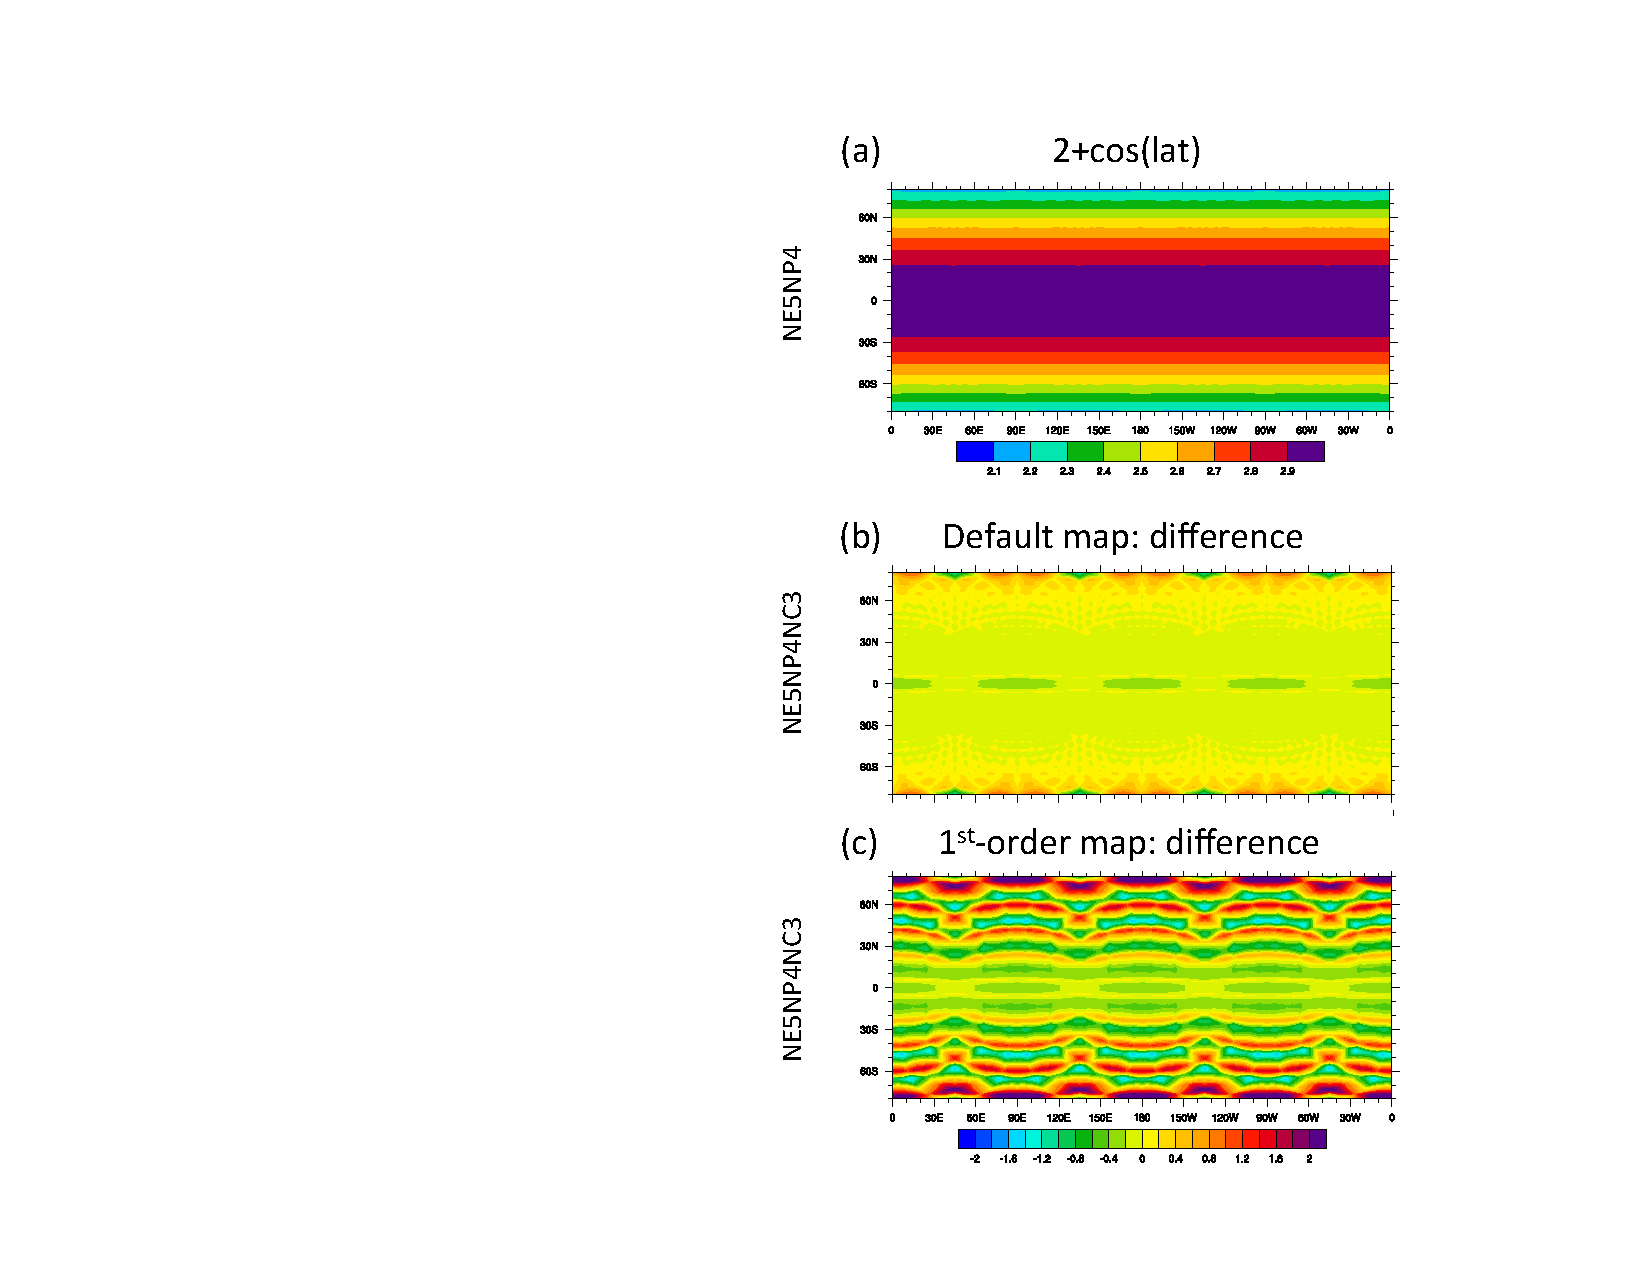
\includegraphics[width=19pc,angle=0]{figs/idealized-mapping-tests-smooth-field.pdf}\\
\caption{(a) Smooth function ($2+\cos(\theta)$) initialized on the $NE5NP4$ GLL grid. (b) and (c) show the difference between the interpolated field and the analytical value at the physics grid cell center. The interpolation is from the $NE5NP4$ GLL grid to the NE5NP4NC3 physics grid (both have an approximate grid spacing of $6^\circ$). In (b) the interpolation algorithm is the default algorithm that is higher-order for smooth fields, shape-preserving, consistent, and mass-conservative. (c) is the same as (b) but using the first-order mapping method. All data has been bilinearly interpolated to a $1^\circ$ regular latitude-longitude grid for plotting.}\label{fig:remap-smooth-field}
\end{figure}
\begin{figure}[t]
\noindent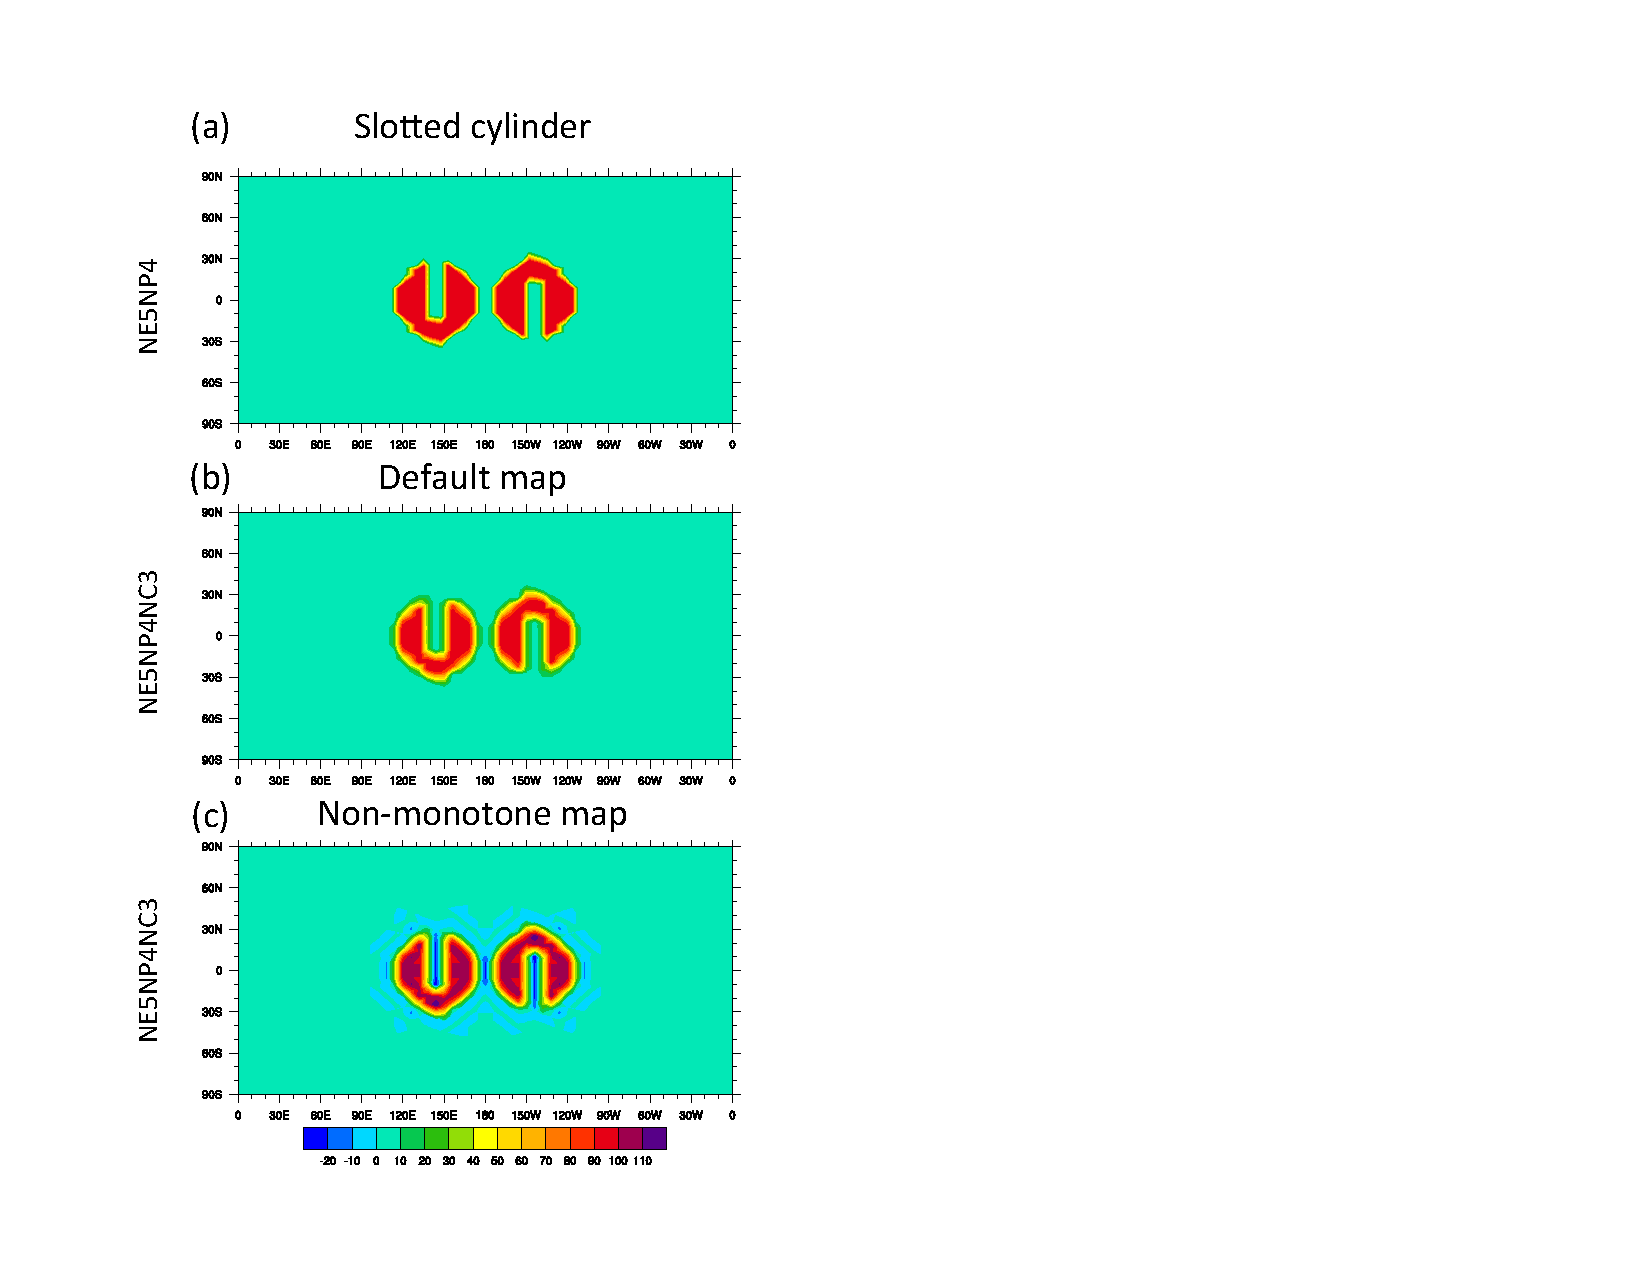
\includegraphics[width=19pc,angle=0]{figs/idealized-mapping-tests-slotted-cylinder.pdf}\\
  \caption{(a) Slotted-cylinder distribution initialized on on the $NE5NP4$ GLL grid (approximately $6^\circ$ resolution). (b) Default mapping of the $NE5NP4$ GLL grid data to the physics grid $NE5NP4NC3$. (c) Same as (b) but using the non-monotone map. All data has been bilinearly interpolated to a $1^\circ\
$ regular latitude-longitude grid for plotting.}\label{fig:remap-slotted-cylinder}
\end{figure}
The low-order map is inaccurate for smooth fields (see Figure \ref{fig:remap-smooth-field}c) and the high-order map is not shape-preserving for, e.g., discontinuous fields (see Figure \ref{fig:remap-slotted-cylinder}c). To avoid using the low-order map in areas where the field is smooth and violation of shape-preservation in areas where the field is not smooth, we linearly combine the two maps in each element:
\begin{equation}
\bm{\mathsf{A}}^{(opt)}=\left[ \alpha^{(opt)} \bm{\mathsf{A}}^{(sp)}+(1-\alpha^{(opt)})\, \bm{\mathsf{A}}^{(un)}\right],\label{eq:opt}
\end{equation}
%so that shape-preservation is not violated and the map retains high-order accuracy where possible.
where $\alpha^{(opt)}$ is the smallest value of $\alpha^{(opt)}$ (so that the high-order map is given as much weight as possible) that guarantees no overshoots or undershoots:
\begin{eqnarray}
\psi_k&\le &\max(\phi_1,...,\phi_{np\times np}), \quad k=1,...,nc\times nc,\label{eq:overshoot}\\
\psi_k&\ge &\min(\phi_1,...,\phi_{np\times np}), \quad k=1,...,nc\times nc.\label{eq:undershoot}
\end{eqnarray}
The value of $\alpha^{(opt)}$ is computed as follows. Assume that there is an overshoot for physics grid cell $k$. We wish to find the value of $\alpha_k$ so that
\begin{equation}
\alpha_k \psi_k^{(sp)}+(1-\alpha_k) \psi_k^{(un)}=\max(\phi_1,...,\phi_{np\times np}),
\end{equation}
which yields
\begin{equation}
\alpha_k = \frac{\max(\phi_1,...,\phi_{np\times np})-\psi_k^{(un)}}{\psi_k^{(un)}-\psi_k^{(sp)}}.
\label{eq:alpha}
\end{equation}
If the absolute value of the denominator in \eqref{eq:alpha} is less than $1.0^{-12}$ then $\alpha_k$ is set to 1. Similarly we compute $\alpha_k$ for undershoots and if there is no under- or over-shoot we set $\alpha_k=0$. The optimal value of $\alpha_k$ that satisfies \eqref{eq:overshoot} and \eqref{eq:undershoot} for all $k$ is
\begin{equation}
\alpha^{(opt)}=\max(\alpha_1, ...,\alpha_{nc\times nc}).
\end{equation}
By optimal we mean the value of $\alpha$ that gives most weight to the unlimited (high-order) map within an element without violating shape-preservation \eqref{eq:overshoot} and \eqref{eq:undershoot}. Note that the linear combination of linear maps is conservative and consistent hence the optimal map \eqref{eq:opt} is conservative, consistent and, by using $\alpha^{(opt)}$, shape-preserving. The limiting process is somewhat similar to \citet{BJ1989} and the flux-corrected transport algorithm \citep{Z1979JCP}.

The mapping of the state variables $\phi$ on the GLL grid to the physics grid is given by
\begin{multline}
\bm{\mathsf{\psi}}=\left[ \alpha^{(opt)} \bm{\mathsf{A}}^{(sp)}+(1-\alpha^{(opt)})\, \bm{\mathsf{A}}^{(un)}\right] \bm{\mathsf{\phi}},
\end{multline}
where $\phi=$ $\Delta p^{(GLL)}$, $\Delta p^{(GLL)}T^{(GLL)}$, $\Delta p^{(GLL)}u_x^{(GLL)}$,$\Delta p^{(GLL)}u_y^{(GLL)}$,$\Delta p^{(GLL)}u_z^{(GLL)}$, $\Delta p^{(GLL)}Q^{(GLL)}$, $\Delta p^{(GLL)}q^{(GLL)}$. The mapped field for, e.g., $\Delta p^{(GLL)}$ is denoted $\psi=\Delta p^{(phys)}$ and similarly for the other variables. The state of the atmosphere is recovered by dividing the mapped fields $\psi$ with pressure-level thickness on the physics grid $\Delta p^{(phys)}$. Since the atmospheric state is mapped from dynamics to physics grid by basically integrating the high-order basis functions, the loss of accuracy is minimized.
%
%
\subsection{Remapping: physics grid $\rightarrow$ GLL grid}
The CAM physics package returns tendencies for temperature $f_T^{(phys)}$, velocity components $(f_u,f_v)^{(phys)}$, water vapor $f_Q^{(phys)}$, other tracers $f_q^{(phys)}$, and surface pressure $f_{PS}^{(phys)}$. The latter forcing is due to the vertical coordinate in CAM-SE being based on `wet' pressure (dry air mass plus the weight of water vapor) so if there is a change in moisture in the column then the `wet' surface pressure  $PS$ changes whereas the dry air mass (surface pressure) remains constant \citep[see section 3.1.8 `Adjustment of pressure to include change in mass of water vapor' in ][]{CAM5}. 

As for the dynamics to physics grid mapping, conservation is important and we therefore mass-weight the variables being mapped. For that $\Delta p$ on the physics and dynamics grid is needed. Mapping the updated surface pressure on the physics grid to the dynamics grid is not desirable: first of all, if there is no tendency on surface pressure then the mapped surface pressure on the GLL grid will be different from the surface pressure on the GLL grid before calling physics. As mentioned before, this is equivalent to having a spurious forcing on $PS$ entirely due to errors in the mapping algorithm. Secondly, conservation properties will result unless the GLL grid surface pressure is overwritten by the mapped $PS$ from the physics grid to the dynamics grid. To ensure conservation and spurious forcing due to mapping errors the following algorithm is adopted for the mass-weighting.

Let $\Delta p_{phys}$ be the updated pressure level thickness returned by physics. Map water-vapor mass $\Delta p_{phys}\, f_Q^{(phys)}$ from the physics to the dynamics grid using a conservative, consistent, and shape-preserving method (see below) resulting in $\Delta p_{phys}\, f_Q^{(phys)}$. This variable is the surface pressure tendency on the GLL grid, $f_{PS}^{(GLL)}$. Now take the surface pressure on the GLL grid before calling physics $p_s^{(GLL)}$ and add the surface pressure tendency $\Delta t PS^{(GLL)}$. This updated surface pressure $p_s^{(GLL)}$ defines the updated pressure-level thicknesses $\Delta p^{(GLL)}$. We use the physics updated pressure level thickness on the physics grid $\Delta p^{(phys)}$ for the mass-weighting of the physics tendencies $f^{(phys)}_i$, where $i=T$, $Q$, $q$, $u_x$. $u_y$, $u_z$, and $\Delta p^{(GLL)}$ for recovering the tendencies after mapping. The velocity forcing is transformed into a Cartesian coordinate system vector as for the dynamics to physics grid mapping.

\subsubsection{Mapping algorithm} [Paul: we are just using low-order map? would it be easy to switch to higher-order?] To build the non-monotone ``first guess'' map from the finite volume physics grid to the finite element dynamics grid, a continuous polynomial reconstruction of degree $n_c-1$ (and order $n_c$) is built that exactly interpolates the volume averaged values in each physics grid element.  For the monotone ``first guess'' map, a second-order bilinear reconstruction is instead employed that interpolates the density field at the center of each finite volume.  In each case the reconstruction is then sampled at each of the Gauss-Lobotto-Legendre nodes of the dynamics grid.

\section{Results}
\begin{figure}[t]
\noindent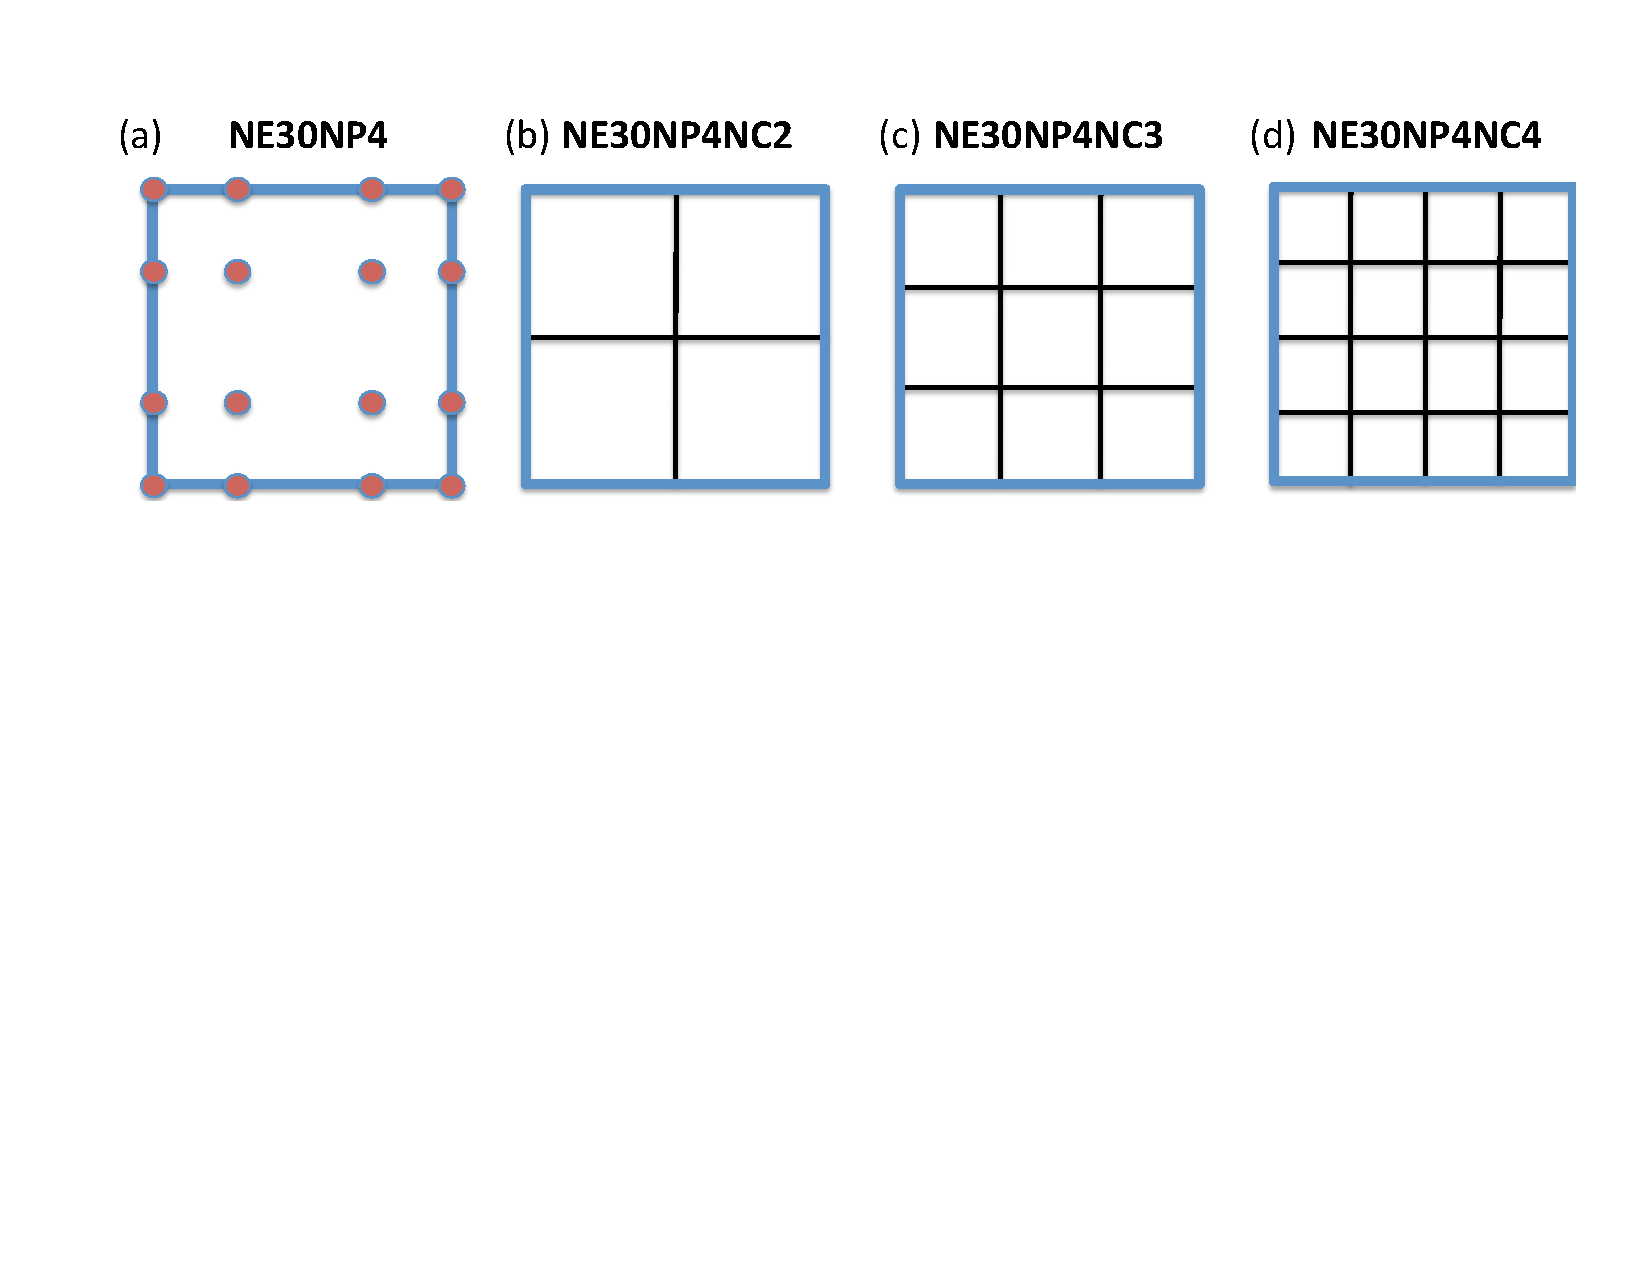
\includegraphics[width=19pc,angle=0]{figs/grids.pdf}\\
  \caption{A graphical illustration of the different physics column configurations: (a) Gauss-Lobatto-Legendre quadrature grid for $np=4$ (filled circles) and (b-d) `equal-area' finite-volume grids of different resolutions ($nc=2,3,4$).}\label{fig:grids}
\end{figure}
%vs

% \section{Section title}
% \subsection{subsection one}
% text...
% \subsection{subsection two}
% \section{Section title}

%%%
\begin{figure}[t]
\noindent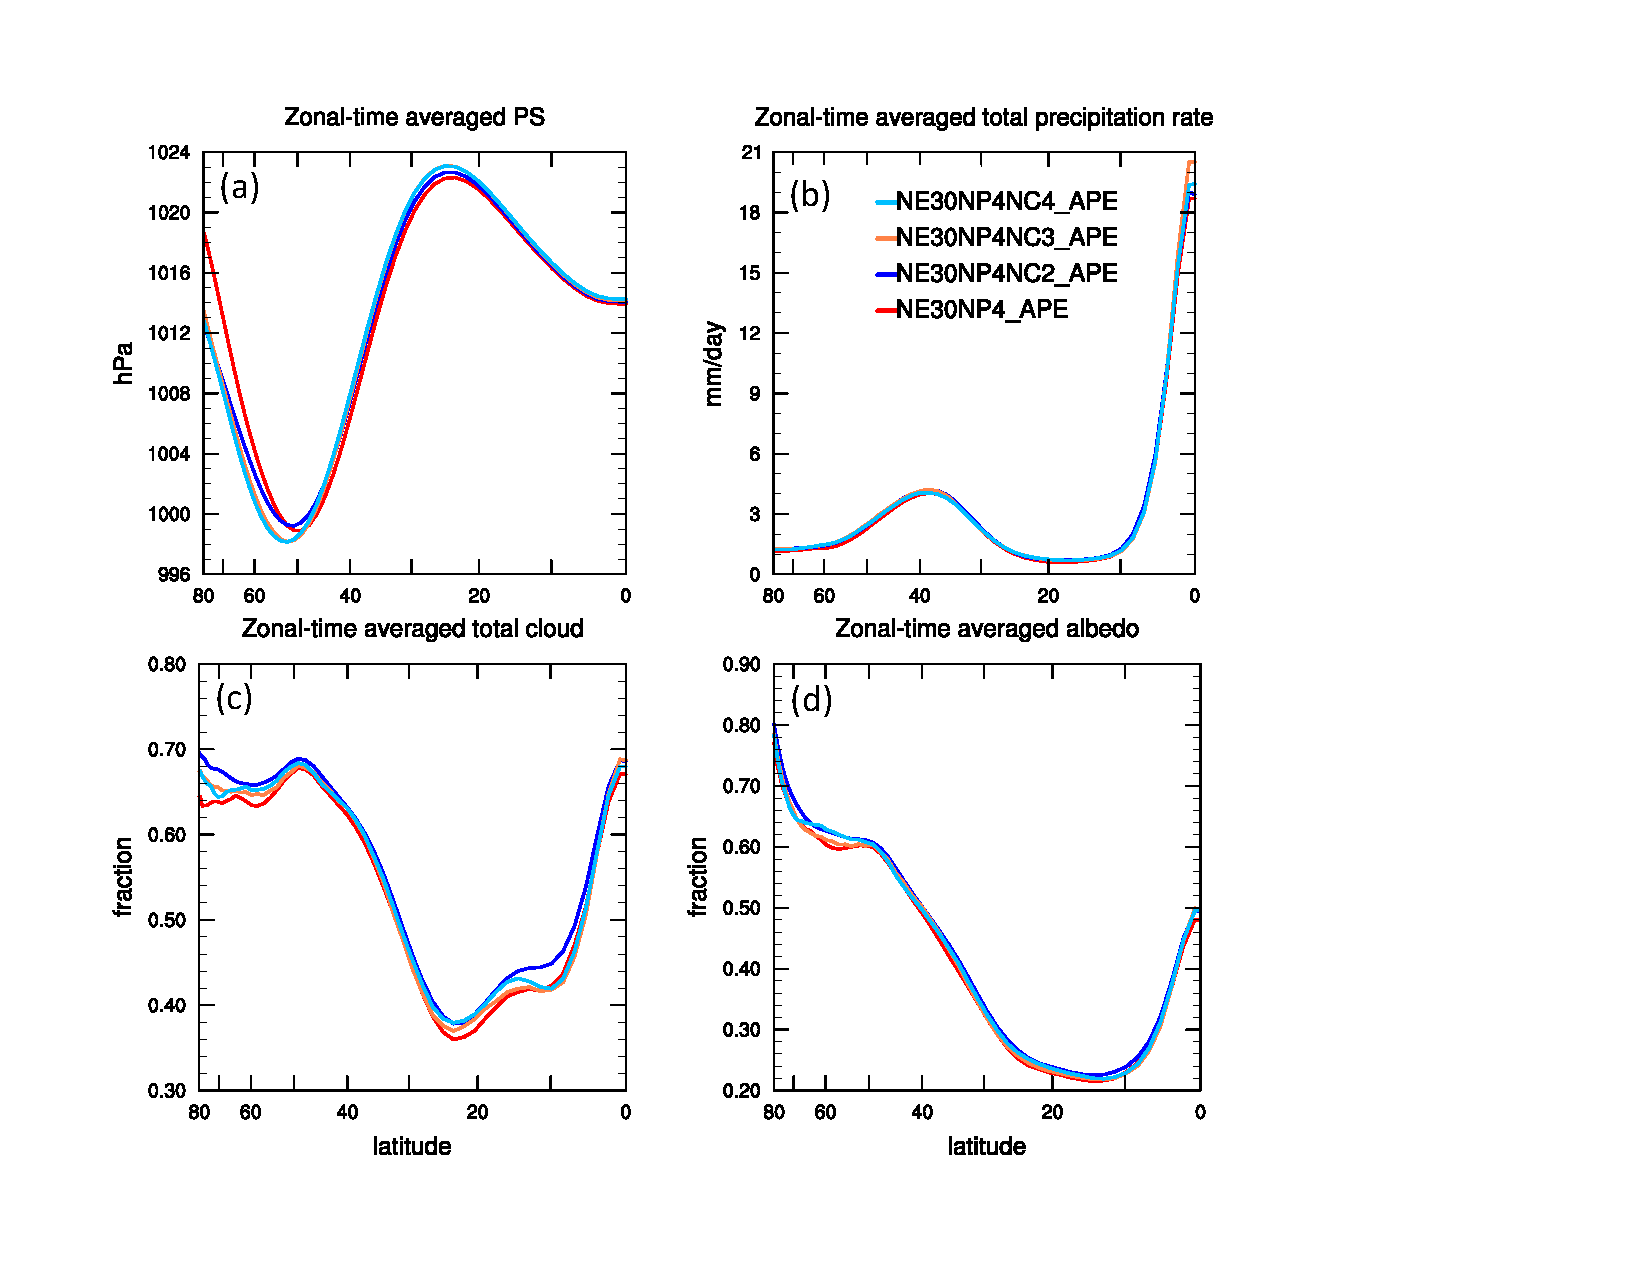
\includegraphics[width=19pc,angle=0]{figs/zonal_time_avg_2d_fields.pdf}\\
\caption{Zonal-time average (a) surface pressure $PS$, (b) total precipitation rate $PRECT$, (c) total cloud fraction $CLDTOT$, and (d) albedo as a function of latitude (from Equator to $80^\circ$N) for the different model configurations. The data has been averaged over a period of 30 months and mapped to a $1.5^\circ$$\times$$1.5^\circ$ regular latitude-longitude grid for analysis.}
\end{figure}

% \subsection{First secondary heading}

% \subsubsection{First tertiary heading}

% \paragraph{First quaternary heading}

%%%%%%%%%%%%%%%%%%%%%%%%%%%%%%%%%%%%%%%%%%%%%%%%%%%%%%%%%%%%%%%%%%%%%
% ACKNOWLEDGMENTS
%%%%%%%%%%%%%%%%%%%%%%%%%%%%%%%%%%%%%%%%%%%%%%%%%%%%%%%%%%%%%%%%%%%%%
%
\acknowledgments
NCAR is sponsored by the National Science Foundation (NSF).

%%%%%%%%%%%%%%%%%%%%%%%%%%%%%%%%%%%%%%%%%%%%%%%%%%%%%%%%%%%%%%%%%%%%%
% APPENDIXES
%%%%%%%%%%%%%%%%%%%%%%%%%%%%%%%%%%%%%%%%%%%%%%%%%%%%%%%%%%%%%%%%%%%%%
%
% Use \appendix if there is only one appendix.
%\appendix

% Use \appendix[A], \appendix}[B], if you have multiple appendixes.
%\appendix[A]

%% Appendix title is necessary! For appendix title:
%\appendixtitle{}

%%% Appendix section numbering (note, skip \section and begin with \subsection)
% \subsection{First primary heading}

% \subsubsection{First secondary heading}

% \paragraph{First tertiary heading}

%% Important!
%\appendcaption{<appendix letter and number>}{<caption>} 
%must be used for figures and tables in appendixes, e.g.,
%
%\begin{figure}
%\noindent\includegraphics[width=19pc,angle=0]{figure01.pdf}\\
%\appendcaption{A1}{Caption here.}
%\end{figure}
%
% All appendix figures/tables should be placed in order AFTER the main figures/tables, i.e., tables, appendix tables, figures, appendix figures.
%
%%%%%%%%%%%%%%%%%%%%%%%%%%%%%%%%%%%%%%%%%%%%%%%%%%%%%%%%%%%%%%%%%%%%%
% REFERENCES
%%%%%%%%%%%%%%%%%%%%%%%%%%%%%%%%%%%%%%%%%%%%%%%%%%%%%%%%%%%%%%%%%%%%%
% Make your BibTeX bibliography by using these commands:
\bibliographystyle{ametsoc2014}
\bibliography{bib}


%%%%%%%%%%%%%%%%%%%%%%%%%%%%%%%%%%%%%%%%%%%%%%%%%%%%%%%%%%%%%%%%%%%%%
% TABLES
%%%%%%%%%%%%%%%%%%%%%%%%%%%%%%%%%%%%%%%%%%%%%%%%%%%%%%%%%%%%%%%%%%%%%
%% Enter tables at the end of the document, before figures.
%%
%
%\begin{table}[t]
%\caption{This is a sample table caption and table layout.  Enter as many tables as
%  necessary at the end of your manuscript. Table from Lorenz (1963).}\label{t1}
%\begin{center}
%\begin{tabular}{ccccrrcrc}
%\hline\hline
%$N$ & $X$ & $Y$ & $Z$\\
%\hline
% 0000 & 0000 & 0010 & 0000 \\
% 0005 & 0004 & 0012 & 0000 \\
% 0010 & 0009 & 0020 & 0000 \\
% 0015 & 0016 & 0036 & 0002 \\
% 0020 & 0030 & 0066 & 0007 \\
% 0025 & 0054 & 0115 & 0024 \\
%\hline
%\end{tabular}
%\end{center}
%\end{table}

%%%%%%%%%%%%%%%%%%%%%%%%%%%%%%%%%%%%%%%%%%%%%%%%%%%%%%%%%%%%%%%%%%%%%
% FIGURES
%%%%%%%%%%%%%%%%%%%%%%%%%%%%%%%%%%%%%%%%%%%%%%%%%%%%%%%%%%%%%%%%%%%%%
%% Enter figures at the end of the document, after tables.
%%
%
%\begin{figure}[t]
%  \noindent\includegraphics[width=19pc,angle=0]{figure01.pdf}\\
%  \caption{Enter the caption for your figure here.  Repeat as
%  necessary for each of your figures. Figure from \protect\cite{Knutti2008}.}\label{f1}
%\end{figure}

\end{document}
